% Chapter 2

\chapter{Methods and Models} % Main chapter title

\label{Chapter2} % For referencing the chapter elsewhere, use \ref{Chapter1} 

\lhead{Chapter 2. \emph{Methods and Models}} % This is for the header on each page - perhaps a shortened title

%----------------------------------------------------------------------------------------


\textit{Graph theory} is a mathematical field applicable to a considerable diversity of complex systems such as markets, ecosystems, computer circuits, and gene-gene interactions [Barabasi, 2009]. A graph is defined as an ensemble of vertices (nodes) that are linked with edges. If the edges connect the nodes in a specified direction, the graph is referred to as \textit{directed}, otherwise \textit{undirected}. Moreover, the edges can be assigned a weight yielding a \textit{weighted} graph. A graph with edges of uniform weight is called an \textit{unweighted} graph.

\textit{Network science} incorporates graph theory applied on a   
distinct complex domain. Unlike classical graph theory, network science primarily deals with real life networks that are large and complex - neither uniformly random nor ordered [RUB10]. The neuro-anatomical and neuro-physiological data sets derived from  DW-MRI and fMRI-BOLD techniques can be constructed as such large-scale complex brain graphs that are undirected and unweighted. Nodes in large-scale brain networks usually represent brain regions, while edges represent anatomical, functional or effective connections (Friston, 1994). 


A brain network can be statistically described in terms of its topology, i.e. solely in terms of its connectivity and independently of spatial positions of nodes and edges. Topological measures described in previous studies capture local and global properties of a network, e.g. local and global efficiency, clustering coefficient, transitivity and small-worldness [LAT01, WAT98, NEW03, HUM08].


Methods of graph theory applied to structural and functional systems have shown that both share typical features of many complex networks [BUL09, RUB09, HEU11, VUK14]. However, the essential features of brain's connectivity still remain ambiguous both for functional and structural maps. This project aims to investigate whether the brain does not behave as a completely random circuitry. This idea will be tested by comparing brain graphs to the randomized networks as it was previously noticed by Bullmore and Bassett [BUL11a]. The majority of random graphs here are inspired by  Erd\H{o}s-R\'{e}nyi type random networks and the configuration model. 
 

In this section, the construction of brain graphs based on empirical functional connectivity matrix (FCM) and anatomical connectivity matrix (ACM) will be first introduced. Then, the topological characteristics of all graphs will be statistically measured and those topological measures will be interpreted neuro-biologically. In particular, it is aimed to explore under which conditions that brain network topologies distinguish from random networks. This approach is expected to provide a deeper insight into the underlying process involved in the observed functional and structural brain connectivity. 


\section{Empirical functional and anatomical connectivity matrices}


\section{The Brain Graph}

The brain graphs considered here are derived from two sets of empirical brain connectivity maps: FCM and ACM obtained from fMRI-BOLD and DW-MRI techniques, respectively. Those data sets represent measurements from $N=90$ cortical and sub-cortical regions labeled with AAL, represented by nodes in the graph. The nodes can be connected to each other by means of "edges". If the graph is constructed on the FCM, edges are interpreted as correlation strengths between the functional BOLD activity of two nodes. If the graph is built on the ACM, an existing edge is considered as the probability of two nodes to be structurally connected by fiber tracks in white matter.

The brain graphs in this project are generated through binarizing the functional connectivity matrix (FCM) and anatomical connectivity matrix (ACM). Binarization here means converting all the values in a given matrix into 1's and 0's via thresholding. Because of the nature of their definition, both empirical data sets have values between 0 and 1, reflecting a correlation strength in case of FCM or a probability value in case of ACM. We arbitrarily define a threshold value $r$ for the strength of correlations in FCM. Then, the values greater and equal to $r$ are assigned the value 1, while others are set to 0. This thresholding is applied by means of the strength of probability value, $p$, for the ACM. The binarized matrix is the basis of brain graph construction, and it is commonly known as \textit{adjacency matrix}. The \textsc{Networkx} software package in \textsc{PYTHON} is used to built graphs given adjacency matrices. Neither the direction of functional or anatomical connectivity between nodes, nor any other values apart from 0 and 1  are encoded in the adjacency matrices,  so that the resulting graphs are considered as "undirected" and "unweighted". In other words, all existing edges are thought to be of uniform weight and nodes interact both ways along an edge connecting them. 

\begin{figure}[htbp]
 %\begin{tabular}{cc}
  \centering
	 \includegraphics[width=90mm,height=52mm]{Figures/bla.eps} 
	 \includegraphics[width=55mm,height=52mm]{Figures/Sample_Adj.eps} 
	 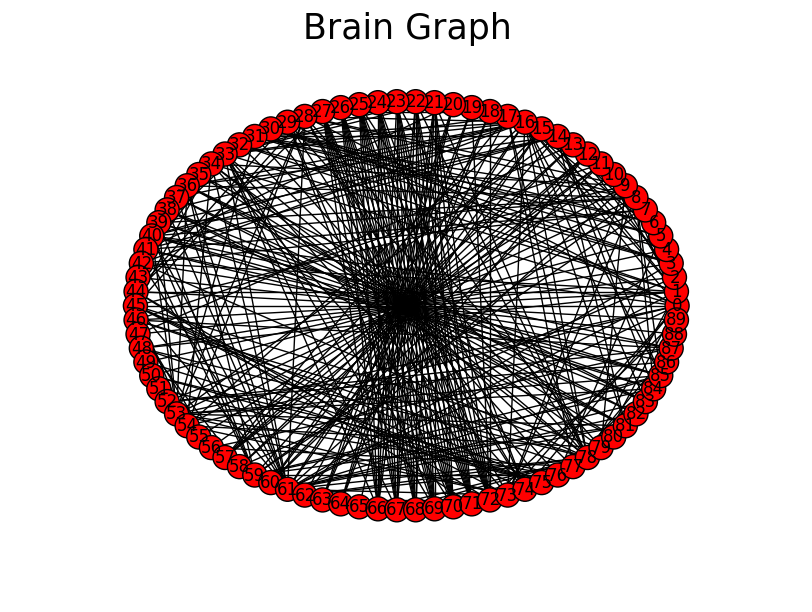
\includegraphics[width=0.50\textwidth]{Figures/brain_graph.png}  
  
    %\includegraphics[width=0.48\textwidth]{Figures/adj_mtx.png} &
	%\includegraphics[width=0.48\textwidth]{Figures/adj_mtx.png} \\
    
    \rule{35em}{0.5pt}
  \caption[Binarizing via thresholding]{How to build a brain graph : The empirical data matrix derived from fMRI-BOLD technique (on the upper left) is binarized via a threshold value $r=0.55$ and its corresponding adjacency matrix is obtained (on the upper right). The black spots represent 1's indicating edges between nodes, whereas the white squares represent 0's implying no connectivity. The brain graph derived from the adjacency matrix (on the bottom) has $N=90$ nodes, edges represent functionally connected node pairs.}
  \label{fig:Binarizing via thresholding}
 %\end{tabular}	
\end{figure}

Figure 2.1 illustrates the exemplary construction of a brain graph exemplary from the FCM. All the correlation values among the cortical and sub-cortical regions in the empirical fMRI-BOLD data lie between 0 and 1. The adjacency matrix (AM) is filled out only with 1's and 0's indicating functionally connected and unconnected nodes, whose correlated BOLD activity is equal to or greater than $r=0.55$. The algorithm \textsc{Networkx} builds the corresponding graph of an adjacency matrix. It should be noted that both FCM and AM are symmetric. The AM obtained from an ACM would look similar, but would represent the probability of two nodes to be anatomically connected above a predefined threshold $p$. 

The following sections will cover randomization methods reshuffling the brain graphs and introduce some of the topological concepts characterizing brain graphs as well as random networks.



\section{Randomization Methods}





\subsection{Erd\H{o}s-R\'{e}nyi Type Randomization}

Given total number of nodes $N$ and a probability $P$, Paul Erd\H{o}s and Alfr\'{e}d R\'{e}nyi produced an undirected graph $G(N,P)$, in which the presence of any edge between two nodes is assigned with probability $P$. 
One can generalize the total number of edges $L$ in an  Erd\H{o}s-R\'{e}nyi type random graph as the following: $\binom {N} {2}P$, pointing out a binomial distribution for the edges per node.

It is possible to improve new randomization tools with adaptations in Erd\H{o}s-R\'{e}nyi method, i.e. given $N$ and $L$, an intended graph $G(N,L)$ can be picked uniformly random out of set of all potential graphs having $N$ nodes and $L$ edges. The probability for a graph to be picked among all the others is $\frac{L}{\binom {N}{2}}  $. One can study the relevance of $G(N,P)$ and $G(N,L)$ even more detailed, but for the sake of simplicity, Erd\H{o}s-R\'{e}nyi model will not discussed further here.

\begin{figure}[htbp]
 %\begin{tabular}{cc}
  \centering
	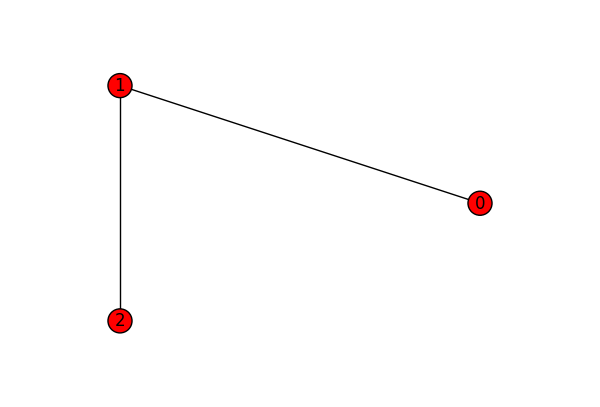
\includegraphics[width=0.30\textwidth, height=40mm]{Figures/f1.png}  
	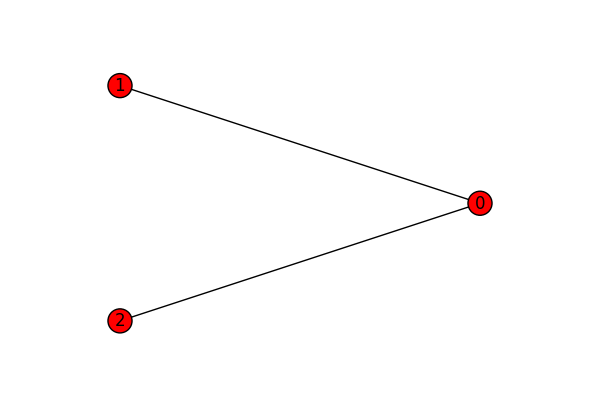
\includegraphics[width=0.30\textwidth, height=40mm]{Figures/f2.png} 
    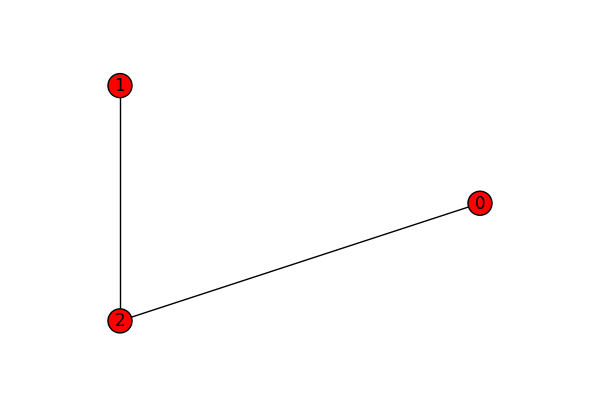
\includegraphics[width=0.30\textwidth, height=40mm]{Figures/f3.png}

    \rule{35em}{0.5pt}
  \caption[Erdos-Renyi Example]{An illustration to the set of all $G(N,L)$ type random graphs with $N=3$ and $L=2$.}
  \label{fig:Erdos-Renyi Example}
 %\end{tabular}	
\end{figure}

Figure 2.2 illustrates all possible graphs having 3 nodes ans 2 edges in total. One of those 3 simple graph is chosen uniformly random for the $G(N,L)$ randomization type means that each graph is chosen with probability $P=\dfrac{1}{3}$.  

The $G(N,L)$ type randomization is the first method used to derive random graphs from the adjacency matrices of FCM and ACM in this project. Both matrices have $N=90$ nodes, however $L$ changes at each brain graph according to the applied threshold and probability level, therefore it is always recalculated. 

\subsection{Double-Edge-Swap Type Randomization}

The \textit{degree} of a node is defined as the number of edges connected to that node, from now on it will be denoted with $k_i$ for the node $i$. The double-edge-swap method manipulates a given graph by swapping two existing edges among four nodes, while keeping the node degrees fixed. 


\begin{figure}[htbp]
 %\begin{tabular}{cc}
  \centering
	\includegraphics[width=0.8\textwidth, height=40mm]{Figures/s.eps}  
    %\includegraphics[width=0.04\textwidth, height=20mm]{Figures/arrow.png}  
	%\includegraphics[width=0.30\textwidth, height=40mm]{Figures/s2.png} 
    \rule{35em}{0.5pt}
  \caption[Double-Edge-Swap Example]{Swapping edges between 4 nodes}
  \label{fig:Double-Edge-Swap Example}
 %\end{tabular}	
\end{figure}

Figure 2.3 illustrates randomly chosen double edges in a sample graph to be swapped. After the existing edges are removed, the new couple of nodes are rewired. The $k_i$ of each node is the same before and after swapping. The \textit{degree distribution} of a graph is a topological property, which reveals a probability distribution of node degrees over whole graph. Although the randomly constructed graphs with the double-edge-swap method based on the brain graphs of FCM and ACM are expected to have the same degree distribution, it is not a unique property identifying a graph.

\subsection{Configuration Model Randomization}

The \textit{degree sequence} of a graph is either ascending or descending sequence of node degrees in a graph. The configuration model intends to return a random graph with given degree sequence. The ideal concept of this model is to assign edges to the nodes randomly until the desired degree sequence is matched. However, the algorithms practicing the configuration model are not so trivial due to self-loops (node is connected to itself) and parallel edges (duplicating edges), which are both undesirable graph properties in this project. 

\begin{figure}[htbp]
 %\begin{tabular}{cc}
  \centering
	\includegraphics[width=0.50\textwidth, height=60mm]{Figures/c1.png}  
    \rule{35em}{0.5pt}
    \caption[Degree Sequence Definition]{The degrees of the nodes: $k_0 = 2$, $k_1 =1$, $k_2=2$, $k_3=3$ and the degree sequence in non-increasing order in the sample graph : $\{3,\,2,\,2,\,1\}$}
  \label{fig:Degree Sequence Definition}
 %\end{tabular}	
\end{figure}

Figure 2.4 points out the relevance of degree sequence to the node degrees. It should be reminded that the degree distribution and the degree sequence are not the same metrics.  

The configuration model variant used here is the expected-degree-graph method, which has an option to exclude self-loops and parallel edges. This algorithm receives the list of expected degree sequence as input, $(k_u, k_v, k_m, k_l, ...)$, and assigns edges between nodes with a predefined probability $P_{uv}=\dfrac{k_u k_w}{\sum_{i}k_i}$. This tool does not guarantee to construct graphs with exactly the same given degree sequence but with the closest possible sequence.  

\subsection{Preserved-Degree-Distribution Type Randomization}

The \textit{degree distribution} of a network reflects the probability of a node to have a given number of degree \textit{k}. The preserved-degree-distribution method randomizes a given undirected network by rewiring its edges randomly while preserving its degree distribution. The method first chooses four target nodes randomly, then flips the edges between those nodes with the probability of $P=0.5$. The total number of rewirings to be performed is given as an iteration parameter to the method. 

 
\subsection{Partial Randomization}
 
The partial randomization method  reconstructs a graph (say A) with partial rewirings with respect to a second graph (say B) while keeping the degree distribution the same as in A. The analogy of this algorithm is to perform rewirings in the adjacency matrix of A, while avoiding any edge generation which already exist in the B. In other words, the choice of edges to be performed rewirings in A is limited with respect to the B. 

In this project, the functional connectivity (FC) adjacency matrix is partially rewired with anatomical connectivity (AC) adjacency matrix.  This means doing such rewirings among the nodes in FCM, only if these nodes are not structurally connected in the brain at above a probability value. The same procedure is done to randomize AC adjacency matrix partially with respect to FC adjacency matrix.  This time such nodes in ACM are rewired, that do not functionally correlated above a given threshold.   

\begin{figure}[htbp]
 %\begin{tabular}{cc}
  \centering
	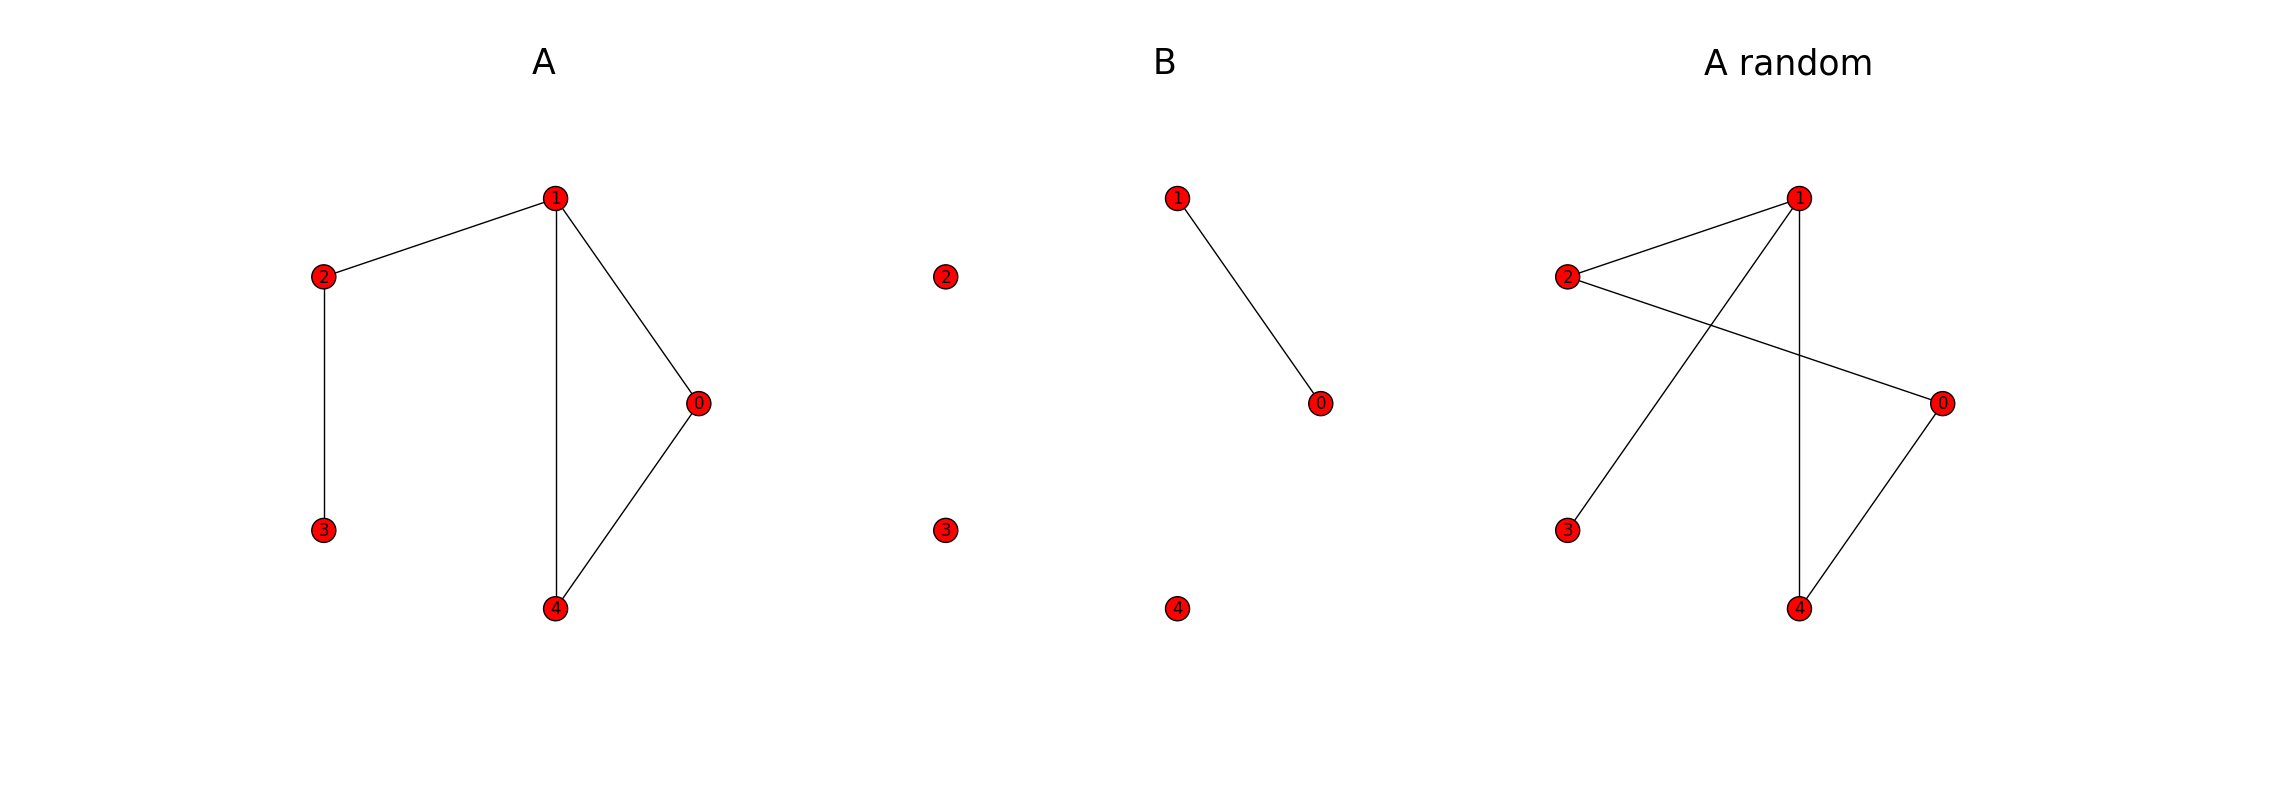
\includegraphics[width=\textwidth, height=55mm]{Figures/p1.png}  
    \rule{35em}{0.5pt}
    \caption[Partial Randomization Example]{Graph A is performed a partial randomization with respect to graph B. While the partial randomization tool rewires edges in A, it avoids creating such edges that exist in B.}
  \label{fig:Partial Randomization Example}
 %\end{tabular}	
\end{figure}

The brain graph and randomly generated graphs will be identified in terms of their topological properties in the following sections. For simplicity the abbreviations are introduced in the table below. 

\begin{table}[h]
\begin{center}
\caption[Abbreviations]{Abbreviations for the brain graph and the randomly constructed graphs. }
\begin{tabular}{ l | c | r }
  Abbreviation & Description & method \\
  \hline  \hline                     
  R0 & the brain graph						  & \textsc{networkx} \\ \hline
  Ra & Erd\H{o}s-R\'{e}nyi, G(N,L)            & \textsc{networkx} \\ \hline
  Rd & double-edge-swap            			  & \textsc{networkx} \\ \hline
  Rg & configuration model       			  & \textsc{networkx} \\ \hline
  Rh & preserved-degree-distribution		  & \textsc{BCT} 	 \\ \hline
  Rk & partial randomization            	  & \textsc{BCT} 	 \\ \hline  
  \hline  
\end{tabular}
\label{table:Abbreviations}
\end{center}
\end{table}	

\section{Network Characterizations}

\subsection{Network Density}
The \textit{average degree} $\langle k \rangle$ of a network indicates the ratio of total number of edges $L$ to total number of nodes $N$ in a graph. 

\begin{equation}
\langle k \rangle = \frac{2L}{N}
\end{equation}

It should be noted that in order to not count each link twice, the total number of edges is divided by $N/2$ instead of $N$. The \textit{density} $D$ of a network is a scaled version of average degree measurement. It is formulated as the ratio between $L$ and maximum number of possible edges ${N \choose 2}$. 

\begin{equation}
D = \frac{2L}{N(N-1)}
\end{equation}	

The measure of network density can be referred as the total \textit{wiring cost} of the network [RUB10]. The degree, average degree and network density are the key ingredients to characterize the topology of a network further. It has even related clinical evidence that reductions in nodal degree have been associated with greater severity of local amyloid deposition in patients with Alzheimer's disease [Buckner et al. 2009]. 

\begin{figure}[htbp]
 %\begin{tabular}{cc}
  \centering
	\includegraphics[width=0.48\textwidth, height=55mm]{Figures/Network_Density_Fnc.eps}
	\includegraphics[width=0.48\textwidth, height=55mm]{Figures/Network_Density_Stru.eps}  
    \rule{35em}{0.5pt}
    \caption[Network Density]{Network density of the brain graphs and random graphs of FCM (on the left) and ACM (on the right). The abbreviations are chosen as described in Table 1.}
  \label{fig:Network Density}
 %\end{tabular}	
\end{figure}


The network density $D$ is presented as probability values lying between 0 and 1 for all the graphs in corresponding threshold $r$ and $p$ ranges. The random networks are built in such ways that they have the same number of $N$ and almost the same $D$ as in the brain graphs. However, the $D$ is not a unique metric identifying a network.

All networks for FCM and ACM seem to be densely connected at lower $r$ and $p$. The brain graph and randomized graphs of FCM follows an inverse sigmoidal $D$ pattern with decreasing threshold $r$. The $D$ decreases slower for the ACM graphs graph with the ascending probability $p$. It should be noted that all the graphs have almost the same $D$ values. 

Functional networks are likely to be denser than anatomical networks, as they will typically contain numerous connections between anatomically unconnected regions [DAM09]. 

\subsection{Average Clustering Coefficient}
    
The \textit{average clustering coefficient} $C$ of a network is calculated through individual clustering coefficients $C_i$ of single nodes,

\begin{equation}
C = \frac{1}{n} \sum\limits_{i\epsilon N}C_i = \frac{1}{n}\sum\limits_{i\epsilon N} \frac{2t_i}{k_i(k_i -1)}
\end{equation} 

where $t_i$ is the number of triangles around node $i$, $k_i$ is the degree of node $i$ [WAT98]. The clustering coefficient is a measure of segregation, that is the ability for specialized processing to occur within densely interconnected groups of brain regions [RUB10]. It reveals how the individual nodes in a graph cluster together; how many neighbors of a node are neighbors of each other. 

\begin{figure}[htbp]
 %\begin{tabular}{cc}
  \centering
	\includegraphics[width=0.48\textwidth, height=55mm]{Figures/Clustering_Coefficient_Fnc.eps}
	\includegraphics[width=0.48\textwidth, height=55mm]{Figures/Clustering_Coefficient_Stru.eps} 
    \rule{35em}{0.5pt}
    \caption[Clustering Coefficient]{Average clustering coefficient of the brain graphs and random graphs of FCM (on the left) and ACM (on the left). }
  \label{fig:Clustering Coefficient}
 %\end{tabular}	
\end{figure}

Clustering coefficient of a node $C_i$ is a measure of local connectivity and is highly correlated with the local efficiency of the information transfer [LAT01]. The $C_i$ is formulated as the ratio of $t_i$ over all possible edges of the node $i$; ${k_i \choose 2} $. The average clustering coefficient $C$ is a normalized version of $C_i$ for the whole network, yielding now a global property. All $C$ values are between 0 and 1. Figure 2.7 shows that at lower threshold, the nodes tend to cluster more due to higher number of existing edges. The empirically obtained brain networks of FCM and ACM have the highest $C$ compared to random graphs. The local information transfer seems to be more efficient in the brain graphs.  The randomized graphs of ACM $Ra$, $Rd$, $Rh$ and $Rk$ share more nodes with lower degrees compared to $R0$.

\subsection{Transitivity}

Transitivity is a similar measure to the clustering coefficient, it is also a measure for the segregation in the network.  The corresponding equation represents the transitivity of a network (Newman, 2003):
	
\begin{equation}
 T = \frac{\sum\limits_{i \epsilon N} 2 t_i}{\sum\limits_{i \epsilon N}k_i (k_i - 1)}
\end{equation}	

If a node has links to two other nodes, transitivity inquires whether those two other nodes are also connected to each other. Transitivity resembles clustering coefficient, however, it is defined only for the whole network rather than single nodes. 

\begin{figure}[htbp]
 %\begin{tabular}{cc}
  \centering
	\includegraphics[width=0.48\textwidth, height=55mm]{Figures/Transitivity_Fnc.eps}
	\includegraphics[width=0.48\textwidth, height=55mm]{Figures/Transitivity_Stru.eps} 
    \rule{35em}{0.5pt}
    \caption[Transitivity]{Transitivity of the brain graphs and random graphs of FCM (on the left) and ACM (on the left). }
  \label{fig:Transitivity}
 %\end{tabular}	
\end{figure}


Transitivity is one of severe shortcomings that real world networks and random networks strongly differ [NEW10]. Transitivity difference between brain graphs and random graphs observed to be more distinguishable than $C$ difference between brain graphs and random graphs when Figure 2.8 is compared to Figure 2.7. 



\section{FitzHugh-Nagumo Model for Neuronal Activity Simulation}

\section{Balloon-Windkessel Model for BOLD Activity Simulation} 
 
%----------------------------------------------------------------------------------------
